\documentclass[10pt]{report}

\usepackage[utf8]{inputenc} % Required for inputting international characters
\usepackage[T1]{fontenc} % Output font encoding for international characters
\usepackage[demo]{graphicx} % images % get rid of [demo] for black box removal
% \usepackage{graphicx} % images % get rid of [demo] for black box removal
\usepackage{fancyhdr} % headers and footers
\usepackage{parskip} % paragraph
\usepackage{geometry} % shapes
\usepackage{hyperref} % Links
\usepackage{pdflscape} % making a page landscape
\usepackage{xcolor}
\usepackage[shortlabels]{enumitem}
\usepackage{multirow}
\usepackage{listings}
\usepackage{float} % to place figures in place

\graphicspath{{../images/}}

% margins and page size
\geometry{
a4paper,
left=30mm,
top=25mm,
right=30mm,
bottom=25mm
}

\lstset{
  basicstyle=\ttfamily,
  columns=fullflexible,
  frame=single,
  breaklines=true,
  postbreak=\mbox{\textcolor{red}{$\hookrightarrow$}\space},
}

\begin{document}

\begin{titlepage}
\center
{\huge\bfseries Computer Graphics 

Aum Patel
}

\end{titlepage}
\tableofcontents
\chapter{Question 1 - Geometry and vertex attributes}

Y-axis up, X axis left to right and Z axis towards you is a Right handed coordinate system. I have proven this by using my right-hand with the X-axis being on the thumb, the Y-axis being on the first finger and the Z-axis being on my middle finger and rotating it to meet the 3 requirements. You cannot rotate the left hand to do this.

\begin{figure}[H]
    \centering
    \fbox{\includegraphics[width = 5cm ]{Right_Hand_Axis.png}}
    \caption{Image of hand with axis labeled.}
\end{figure}

I decided to draw out the model I was going to make in Blender first and then place the vertices on top of it. 

The colors of the axis are consistent in all images: \textcolor{red}{Red : X} , \textcolor{green}{Green : Y} , \textcolor{blue}{Blue : Z}

\begin{figure}[H]
    \centering
    \fbox{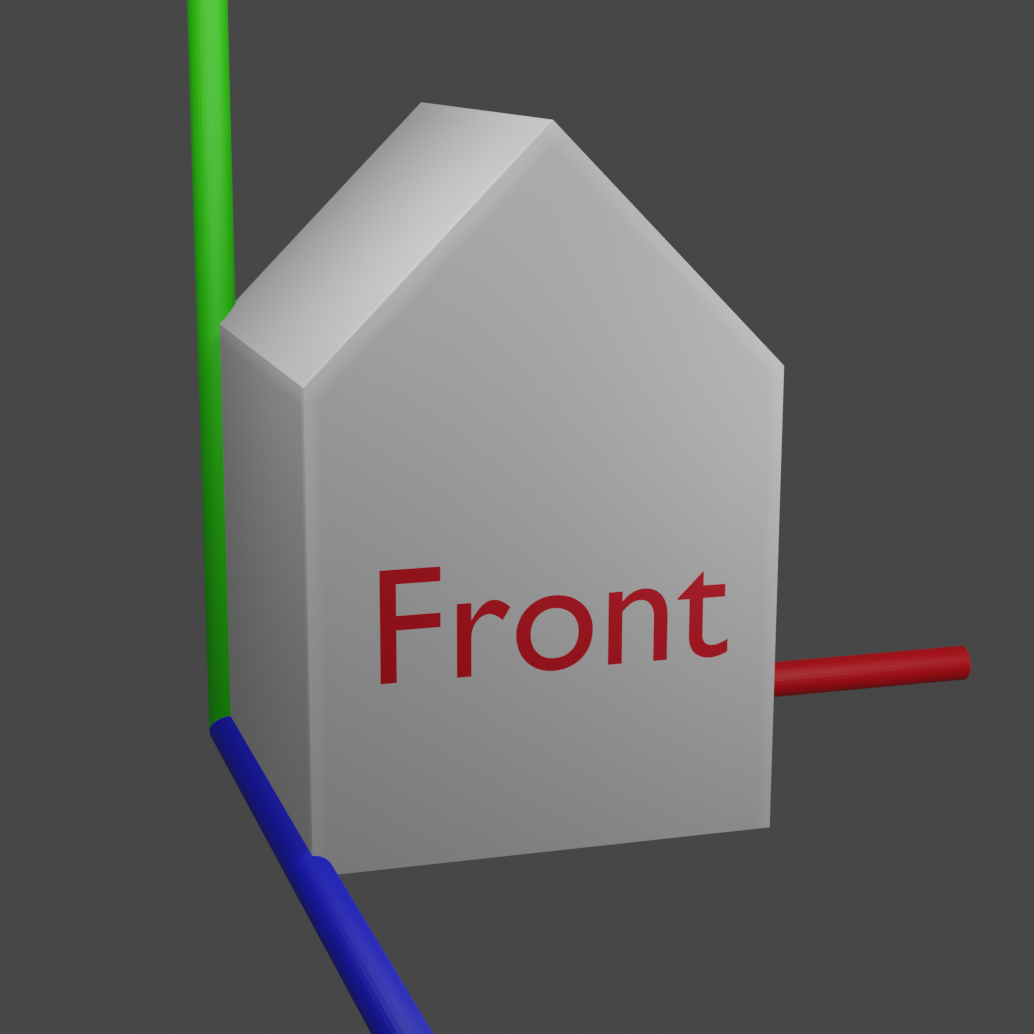
\includegraphics[width = 5cm ]{house_blender.png}}
    \caption{House in blender with drawn axis.}
\end{figure}

I chose the bottom vertex on the rear left of the house as the origin as I would only have to work with positive numbers for the rest of the vertices, and they would also be round numbers (except for the roof) as I am going to make the house with a square base of 1x1. 

Below is a wireframe view of the same house with the coordinates labeled.
\begin{figure}[H]
    \centering
    \fbox{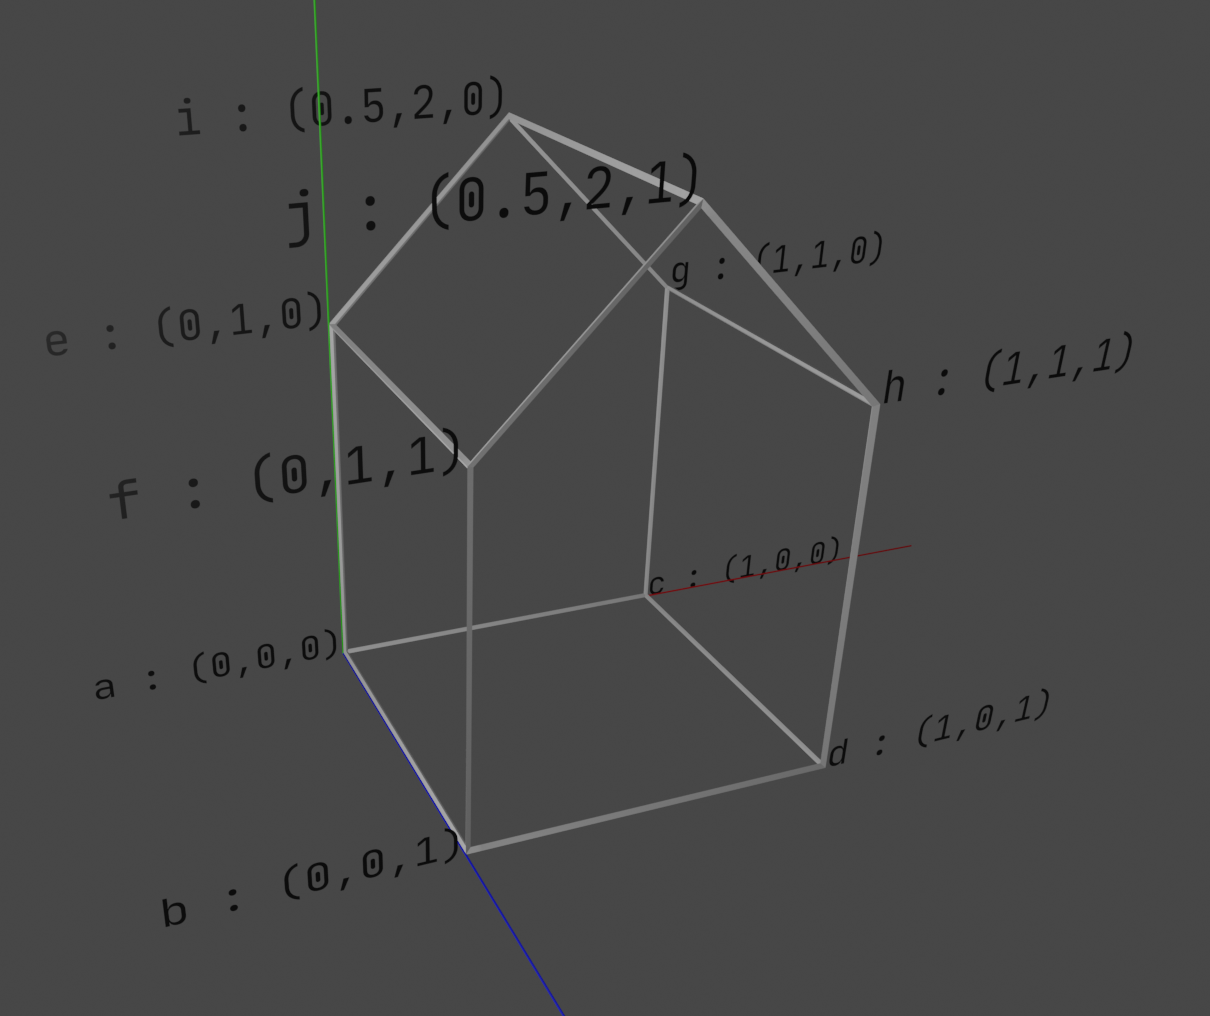
\includegraphics[width = 10cm ]{house_blender_wireframe_with_coord.png}}
    \caption{House in blender with wireframe and coordinates.}
\end{figure}

Coordinates for the vertices:
\begin{enumerate}[(a)]
    \item (0, 0, 0)
    \item (0, 0, 1)
    \item (1, 0, 0)
    \item (1, 0, 1)
    \item (0, 1, 0)
    \item (0, 1, 1)
    \item (1, 1, 0)
    \item (1, 1, 1)
    \item (0.5, 2, 0)
    \item (0.5, 2, 1)
\end{enumerate}

16 triangles will be used to make up the house, and there will be normals that are shared between them.

% Left
% (a, b, f)
% (a, f, e)

% Front
% (b, h, f)
% (b, d, h)
% (f, h, j)

% Right
% (d, g, h)
% (d, c, g)

% Back
% (c, e, g)
% (c, a, e)
% (g, e, i)

% Base
% (a, c, b)
% (b, c, d)

% Roof Left
% (e, j, i)
% (e, f, j)

% Roof Right
% (h, i, j)
% (h, g, i)



I calculated the vector normals by using the following equation:

If we have 3 vectors that make up a a triangle in an anti-clockwise manner: \(V0, V1, V2\), to calculate the normal facing outwards we do:

\(A = V1 - V0\)  |  \(B = V2 - V0\)

\(Normal = A \times B\)

Doing this with the first triangle on the table (triangle on the left face of the house) give you:

\(A = (0, 0, 1) - (0, 0, 0)\) \\ \(A = (0, 0, 1)\)

\(B = (0, 1, 1) - (0, 0, 0)\) \\ \(B = (0, 1, 1)\)

\(Normal = (0, 0, 1) \times (0, 1, 1)\) \\ \(Normal = (-1, 0, 0)\)

I confirmed this calculation to be correct by looking at the shape itself in 3D space, and \((-1, 0, 0)\) is the normal that would be correct.

I had no need to normalise the vectors as they output from the cross product was a sensible number.

Same calculation is done for the rest of the sides, triangles facing the same direction will have the same surface normals.

\begin{table}
    \begin{tabular}{|l|l|} 
    \hline
    \textbf{ Triangles } & \textbf{Normals }              \\ 
    \hline
    (a, b, f)            & \multirow{2}{*}{(-1, 0, 0)}    \\
    (a, f, e)            &                                \\ 
    \hline
    (b, h, f)            & \multirow{3}{*}{(0, 0, 1)}     \\
    (b, d, h)            &                                \\
    (f, h, j)            &                                \\ 
    \hline
    (d, g, h)            & \multirow{2}{*}{(1, 0, 0)}     \\
    (d, c, g)            &                                \\ 
    \hline
    (c, e, g)            & \multirow{3}{*}{(0, 0, -1)}    \\
    (c, a, e)            &                                \\
    (g, e, i)            &                                \\ 
    \hline
    (a, c, b)            & \multirow{2}{*}{(0, -1, 0)}    \\
    (b, c, d)            &                                \\ 
    \hline
    (e, j, i)            & \multirow{2}{*}{(-1, 0.5, 0)}  \\
    (e, f, j)            &                                \\ 
    \hline
    (h, i, j)            & \multirow{2}{*}{(1, 0.5, 0)}   \\
    (h, g, i)            &                                \\
    \hline
    \end{tabular}
\end{table}

\newpage

To write the .obj file, I have to change the alphabetical indices that I have been using into numerical. I have rounded the numbers to 6 decimal places. I have the same number of vertex normals as vertices as I decided to make the shape smooth shaded. 

NOTE THE VERTEX NORMALS HAVE NOT BEEN NORMALISED.


\begin{enumerate}[v]
    \item 0 0 0 % 1 a
    \item 0 0 1 % 2 b
    \item 1 0 0 % 3 c
    \item 1 0 1 % 4 d
    \item 0 1 0 % 5 e
    \item 0 1 1 % 6 f
    \item 1 1 0 % 7 g
    \item 1 1 1 % 8 h
    \item 0.5 2 0 % 9 i
    \item 0.5 2 1 % 10 j
\end{enumerate}     
% normalize vector (-0.333333333333, -0.333333333333, -0.333333333333)
% normalize vector (-0.333333333333, -0.333333333333, 0.333333333333)
% normalize vector (0.333333333333 ,-0.333333333333,-0.333333333333)
% normalize vector (0.333333333333 ,-0.333333333333,0.333333333333)
% normalize vector (-0.66666666667, 0.1666666667,-0.333333333333)
% normalize vector (-0.66666666667, 0.1666666667,0.333333333333)
% normalize vector (0.0, 0.1666666667, -0.333333333333)
% normalize vector (0.0, 0.1666666667, 0.333333333333)
% normalize vector (0.0, 0.333333333333, -0.333333333333)
% normalize vector (0.0, 0.333333333333, 0.333333333333)
\begin{enumerate}[vn]
    \item -0.333333 -0.333333 -0.333333 % 1 a
    \item -0.333333 -0.333333 0.333333 % 2 b
    \item 0.333333 -0.333333 -0.333333 % 3 c
    \item 0.333333 -0.333333 0.333333 % 4 d
    \item -0.666667 0.166667 -0.333333 % 5 e
    \item -0.666667 0.166667 0.333333 % 6 f
    \item 0.0 0.166667 -0.333333 % 7 g
    \item 0.0 0.166667 0.333333 % 8 h
    \item 0.0 0.333333 -0.333333 % 9 i
    \item 0.0 0.333333 0.333333 % 10 j
\end{enumerate}  
usemtl matWall
\begin{enumerate}[f]
    \item 1//1 2//2 6//6
    \item 1//1 6//6 5//5
    \item 2//2 8//8 6//6
    \item 2//2 4//4 8//8
    \item 6//6 8//8 10//10
    \item 4//4 7//7 8//8
    \item 4//4 3//3 7//7
    \item 3//3 5//5 7//7
    \item 3//3 1//1 5//5
    \item 7//7 5//5 9//9
    \item 1//1 3//3 2//2
    \item 2//2 3//3 4//4
\end{enumerate}
usemtl matRoof
\begin{enumerate}[f]
    \item 5//5 10//10 9//9
    \item 5//5 6//6 10//10
    \item 8//8 9//9 10//10
    \item 8//8 7//7 9//9
\end{enumerate}


\chapter{Question 2 - Vertex Buffer Object(VBO) design and transformations}
\begin{center}
\begin{verbatim}
You now have to design a VBO to contain the vertex attributes for your house. Choose a suitable layout for your VBO and list the calls to OpenGL from your client program required to transfer the VBO to the GPU. These should be native OpenGL commands. Do not assume that you have the helper classes from the template. Ensure that you give the correct values for the position and stride for each of the vertex attributes in VBO.

Your house is to be translated so it is centred at a new position on the ground plane, rotated by an angle that is not a multiple of 90º in such a way that the house remains correctly positioned on the ground and scaled to some multiple of its size. Choose your own rotation,translation and scale and provide the calls to glm using a glUtilmatrix stack that will achieve the desired transformation. Also provide the code to transfer this information to the GPU
\end{verbatim}
\end{center}

My single VBO will look like this:
\begin{verbatim}
x y z x y z x y z r g b r g b r g b
\end{verbatim}
which is the standard format, making the attributes tightly packed.

I will add the vertices for the triangles into an array of floats of size 3 * numberOfTriangles, three coordinates per triangle in the counter-clockwise order they should be drawn to render outside, the first two triangles will look like this followed by the rest of the vertices:
triangleVertices[30] = 
\{0, 0, 0,

0, 0, 1

0, 1, 1,

0, 0, 0,

0, 1, 1,

0, 1, 1,

...\}

As the RGB values are in the VBO, I will initialise them as an array of size 30 as well.
triangleColors[30] = 
\{1, 1, 1,

1, 1, 1,

1, 1, 1,

1, 1, 1,

1, 1, 1,

1, 1, 1, 

...\}

Two uint (GLuint) variables will need to be created, one is VAO (will be called \textbf{vao}) and the other is VBO (will be called \textbf{vbo}).

We then call the following functions:
\begin{lstlisting}[language=c]
    // Will have to create two arrays of floats that contain the vertices for all the triangles and the colours for all the triangles both size 10 
    const GLfloat triangleVertices[30] = {...`will have all the vertices here as floats`...}
    const GLfloat triangleColours[30] = {...`will have all the colour data here as floats`...}

    // Will generate a vertex array object (allocate space) and assign it to vao. We pass through a reference so that it will change the variable.
    glGenVertexArrays(1, &vao);

    // Bind the VAO created to the current object
    glBindVertexArray(vao);

    // We then allocate space and generate a vbo, again passing through a reference
    glGenBuffers(1, &vbo)

    // then bind the vbo to the target which is GL_ARRAY_BUFFER
    glBindBuffer(GL_ARRAY_BUFFER, vbo)

    // We pass in the data separately by sub-dividing the buffer, as we would like to allocate vertices and color to the same buffer. This could be done so that you create two separate buffers and VBOs like seen on https://www.khronos.org/opengl/wiki/Tutorial2:_VAOs,_VBOs,_Vertex_and_Fragment_Shaders_(C_/_SDL)#Compilation
    // Here, 0 is the starting index and 30 is the sizeof(triangleVertices)
    glBufferSubData(GL_ARRAY_BUFFER, 0, 30, triangleVertices); // vertices
    
    // Here, 30 is the starting index and 30 is the sizeof(triangleColours)
    glBufferSubData(GL_ARRAY_BUFFER, 30, 30, triangleColours); // colours

    // we will enable the vertex attribute arrays one after the other creating the correct 
    glEnableVertexAttribArray(0);
    
    glEnableVertexAttribPointer(0, 3, GL_FLOAT, GL_FALSE, 0, 0);
    
    
    glEnableVertexAttribArray(1);
    // here the last parameter is a pointer to 30 as that is where the colour data starts in the buffer
    glEnableVertexAttribPointer(0, 3, GL_FLOAT, GL_FALSE, 0, (const GLvoid*) 30);

    
\end{lstlisting}

% This should pass the vertex data to a buffer in the GPU.

Now to transform it and then render the object we will use a glutil::MatrixStack to transform the object.

\begin{lstlisting}[language=c]

    glUtil::MatrixStack matrixStack; // creating the stack
    matrixStack.SetIdentity(); // setting it to an identity matrix

    matrixStack.Push();
        // 14 points on X, 6 Points on Z, so it is still on the ground plane while being on a new positions
        matrixStack.Translate(14, 0, 6);
        // rotating 38 degrees on the y axis
        matrixStack.Rotate(glm::vec3(0, 1, 0), 38);
        // scaling the house by 3.7f uniform points
        matrixStack.Scale(3.7f);


        // now to render the triangles we pass in the vao that we created and then draw it on screen.
        glBindVertexArray(vao);
        glDrawElements(GL_TRIANGLES, , GL_UNSIGNED_INT, 0)
    matrixStack.Pop();

\end{lstlisting}

\chapter{Question 3 - Camera Positioning}

\(\textbf{zNear}\) and \(\textbf{zFar}\) define the distance of the near and far clipping planes. Anything that is in front of the camera but its distance is less than \(\textbf{zNear}\), it will not be displayed; vice versa with \(\textbf{zFar}\), anything in front of the camera but farther away than \(\textbf{zFar}\) will not be shown.

\(\textbf{fovy}\) is the field of view of the camera, giving a bigger number will increase the field of view and display more on screen, decreasing it will compress the image and only show a little portion of it. It is the angle $\theta$ of the separation of the planes on the Y axis. See image I created below that shows it better.

\begin{figure}[H]
    \centering
    \fbox{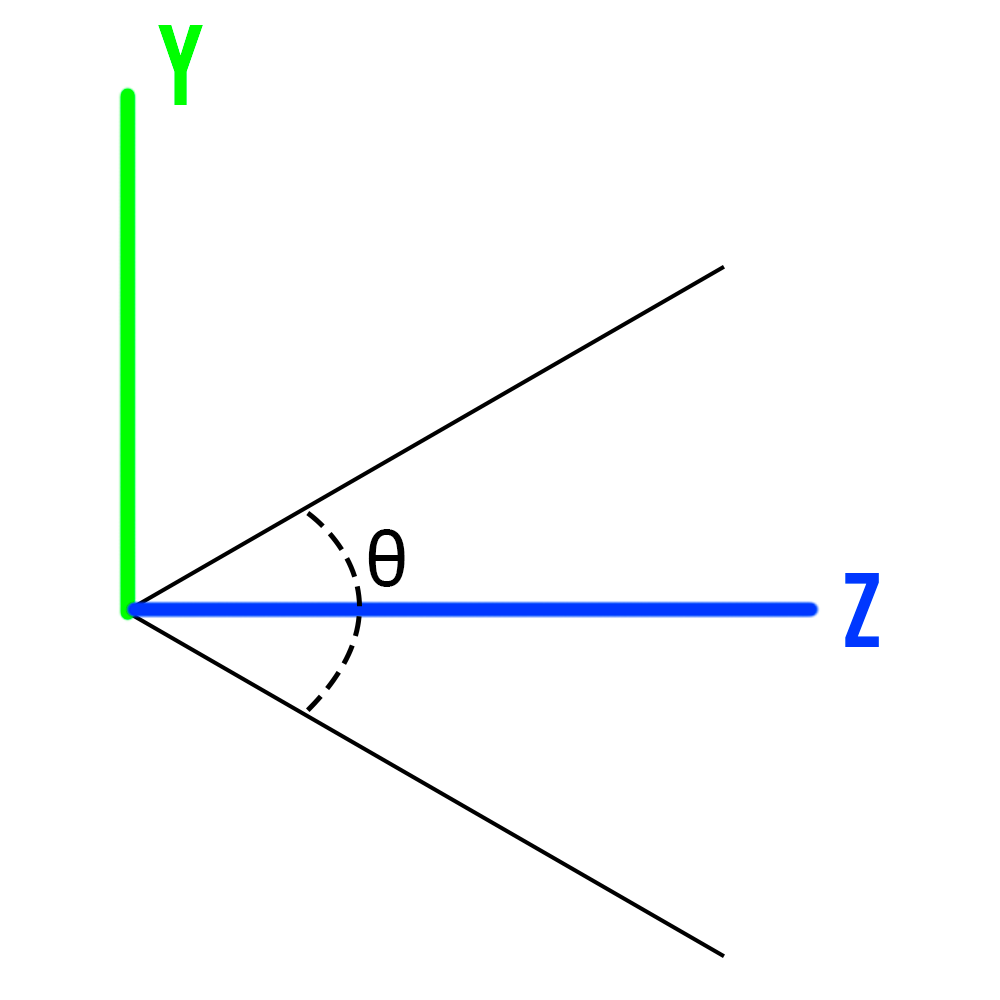
\includegraphics[width = 10cm ]{FOV.png}}
    \caption{Diagram showing what the FOV number/angle means. In this image the two lines are 60$^{\circ}$ apart}
\end{figure}

The \(\textbf{aspect}\) is the ratio between the width (x) and the height (y) of the view, it can also be described as the field of view in the X axis.

Calling \(gluPerspective()\) with these parameters (which are all of type GLdouble) will set up a perspective projection matrix.

I will use the original position for house as seen in question 1 and not the position transformed to in question 2.

I will have the camera's perspective projection matrix be created with the following parameters: 
\begin{lstlisting}[language = c]
    fovy = 60.0 // an appropriate angle that is similar to the human eye
    aspect = 1 // making it square
    zNear = 1 // I do not want objects in front of the camera to clip to early
    zFar = 50 // plenty of room for the far end of the clipping plane.
\end{lstlisting}

Now to position the camera and provide the forward and the up vector. I will position it so that the camera is pointing straight into it and looking at the front of the house.
\begin{lstlisting}[language = c]
    // The house is sitting on the XZ plane and has a total height of 2, so I placed the camera on the center with 1 on the Y axis. As the house goes from 0 to 1 on the X, I decided to place the camera in the center, this being 0.5. As the house already extrudes by 1 on the Z axis, I moved the camera back by 2 extra points to make sure that the house will fit into the FOV, making it 3 on the Z.
    cameraPosition = glm::vec3(0.5f, 1, 3) 

    // the forward is -1 on the Z as it is facing the front of the house that has a normal of (0,0,1)
    cameraForward = glm::vec3(0,0,-1) 

    // the up is going to be positive on the Y as the camera is not angled.
    cameraUp = glm::vec3(0,1,0) 
\end{lstlisting}


There are two methods of rotating the camera around a certain object while always keeping it in the center of view.
One is by creating a Catmull Rom Spline that is a circle around the house.

The other is using sin and cos (using a trig unit circle) over delta time to get the correct positions of X and Z. I will be going with the later method as it seems the most straight forward.

\begin{figure}[H]
    \centering
    \fbox{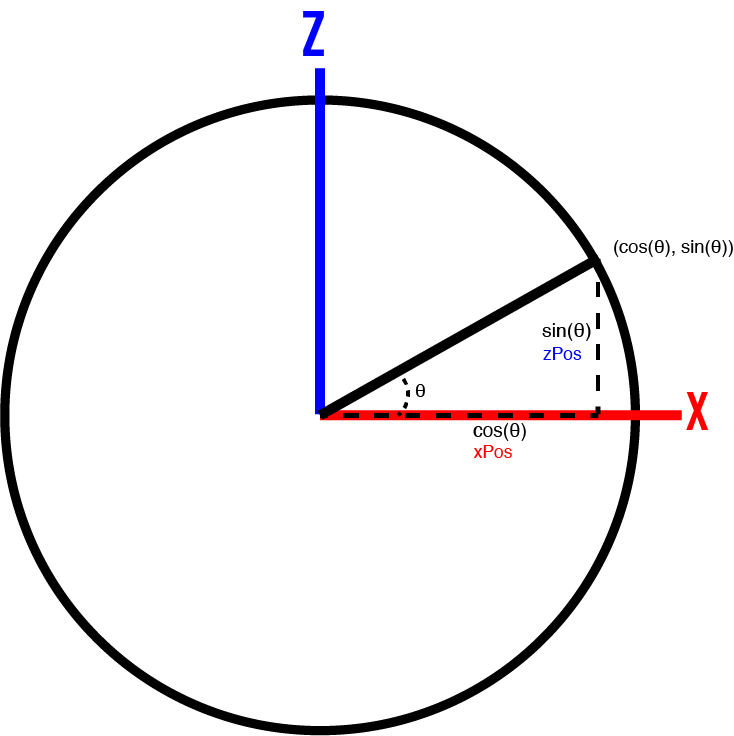
\includegraphics[width = 10cm ]{Trig_Circle.png}}
    \caption{Diagram explaining using the trig unit circle finding out the x and z positions}
\end{figure}


We can use the glm::lookAt() method to get a viewing matrix that will change what is being seen in the world. The following code will be executed every frame, and am assuming delta time \(dt\) is being passed through. The radius will be 10 in this case, and will be offset by the house's position.

\begin{lstlisting}[language = c]
    // set the radius
    radius = 10

    // the height from the house that the camera will be placed at
    auto yPos = 1 + house.position.y // offset by the house's Y

    // house.position is a vec3 with the house's position
    // get the X position 
    auto xPos = (cos(dt) * radius) + house.position.x; // offset by house's X

    // get the Z position
    auto zPos = (sin(dt) * radius) + house.position.z; // offset by house's Z

    cameraPosition = glm::vec3(xPos, yPos, zPos); // will be the vEye in the lookAt

    cameraUp = glm::vec3(0,1,0); // will be the camera up variable

    // updating the view matrix with the new camera data
    // lookAt(eyePosition, viewPoint, cameraUpVector)
    viewMatrix = glm::lookAt(cameraPosition, house.position, cameraUp);

\end{lstlisting}


\chapter{Question 4 - Shader Implementation}


\end{document}